\subsection{Chunked data streaming}

The Erlang NetInf NRS includes two different ways to stream chunked data. The first is the modified version of NetInf that removes the overhead of publishing each chunk to the NRS. The other implementation uses pure NetInf to publish each chunk. Both of them use an HTML5 interface to playback the stream. 

%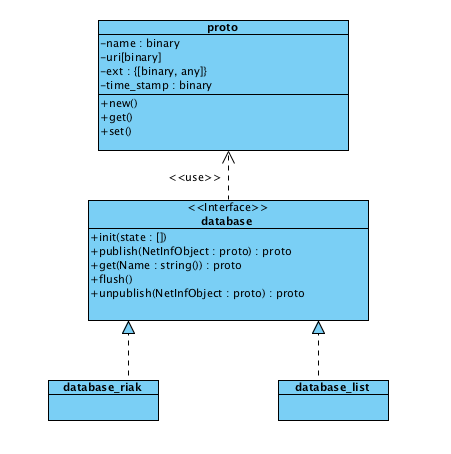
\includegraphics[scale=0.5]{./img/database_api.png}

\subsubsection{Content dispatcher}

To be able to transfer the chunks to the local HTML5 interface a content dispatcher service was added. The difference is that the content dispatcher service serve the NDOs' octects directly through HTTP, that is without the multi-part response as done in the HTTP CL. The module for this is the \textit{nn\_ct\_handler}. This service is spawned when the NRS system starts and runs on port 8078. To request the octects of the NDO \textit{ni:///sha-256-64;abc} pass the url:

\begin{verbatim}
http://localhost:8078/octets/ni%3A%2F%2F%2Fsha-256-64%3Babc 
\end{verbatim}
